% BER+ Board Room — Beschäftigungstiefe briefing for Thomas Graf (Alpine)
% Build: node ../build-report.mjs  OR  npm run graf:report

\documentclass[10pt,a4paper]{article}
\usepackage[utf8]{inputenc}
\usepackage[T1]{fontenc}
\usepackage[margin=1.75cm]{geometry}
\usepackage{graphicx}
\usepackage{booktabs}
\usepackage{hyperref}
\usepackage{parskip}
\usepackage{caption}
\usepackage{subcaption}
\usepackage{xcolor}
\usepackage{tabularx}

\hypersetup{colorlinks=true,linkcolor=blue!70!black,urlcolor=blue!70!black}
\newcommand{\berhub}{\textbf{BER+ Board Room}}
\newcommand{\sectionrule}{\vspace{0.25em}{\color{black!20}\hrule height 0.4pt}\vspace{0.45em}}

\graphicspath{{figures/}}
\setlength{\parskip}{0.4em}
\setlength{\parindent}{0pt}
\captionsetup{font=small,skip=4pt}

\begin{document}

\begin{center}
  {\LARGE Beschäftigungstiefe near Schönefeld}\\[0.25em]
  {\large A business briefing for Thomas Graf's workforce question}\\[0.4em]
  {\normalsize \berhub{} · integrated page \texttt{/beschaeftigung} · IDI S26 · Tian Shao · Yushu Qin · Yi Li}\\[0.15em]
  {\small XU University of Applied Sciences · June 2026}\\[0.3em]
  {\small\textit{Indicative analysis --- not official labour-market statistics}}
\end{center}
\sectionrule

\section*{Executive summary}
After the June 2026 Board Room presentation, \textbf{Thomas Graf} (Alpine Immobilien; BER+ 2.\ Vorsitzender) asked whether firms near Schönefeld employ enough people for new \textbf{Büro/Gewerbe} to succeed.

\textbf{Our reframing.} The question is not mainly about construction crews on site. It is about \textit{Beschäftigungstiefe}: tenant depth, existing jobs in the corridor, and whether firms can recruit \textbf{Fachkräfte} from the wider Berlin--Brandenburg catchment.

\textbf{What we did.} We integrated a dedicated workforce briefing into \berhub{} (\texttt{/beschaeftigung}), linked from the map footer and Briefing tab. The page maps \textbf{215 named employers} from live OpenStreetMap data, cross-references public headcount where available, and applies a transparent \textbf{corridor employment model} for the remaining locations.

\textbf{Headline findings (indicative).}
\begin{itemize}
  \setlength{\itemsep}{0.12em}
  \item \textbf{BB Business Hub} (Alpine proof point): $\sim$50 firms, $\sim$800 employees on campus.
  \item \textbf{FBB} (airport operator): $\sim$2{,}131 employees (2023 annual average, published).
  \item \textbf{643} gewerbe / industrial OSM features in the Schönefeld bbox; \textbf{215} carry a business name.
  \item \textbf{102} sites had no public site-level count --- modelled at \textbf{$\sim$4{,}075 jobs} (point estimates, see below).
  \item \textbf{Corridor footprint} (site-level + modelled + micro-estimates, \textit{excluding} corporate HQs such as DHL global): order of magnitude \textbf{$\sim$11k--14k jobs} mapped as plausible local presence --- transparency before strategy, not a finished GIS.
\end{itemize}

\textbf{Recommendation.} Publish this briefing on the neutral Board Room map; run a \textbf{90-day member validation} with Alpine and 3--5 anchor Mitglieder before any leasing narrative is treated as authoritative.

\section*{0.\ Integration in Board Room}
The final version lives inside the main Next.js app --- not a separate HTML demo.

\begin{figure}[htbp]
  \centering
  \begin{subfigure}[t]{0.48\textwidth}
    \centering
    
\includegraphics[width=\linewidth,keepaspectratio]{fig-app-board-briefing-tab.png}
    \caption*{Briefing tab CTA on the war-room map}
  \end{subfigure}\hfill
  \begin{subfigure}[t]{0.48\textwidth}
    \centering
    
\includegraphics[width=\linewidth,keepaspectratio]{fig-app-header.png}
    \caption*{Dedicated \texttt{/beschaeftigung} page header}
  \end{subfigure}
  \caption{Board Room navigation: footer link \textit{Workforce}, Briefing-panel card, and full-page briefing route.}
\end{figure}

\section*{1.\ Stakeholder question}
\begin{figure}[htbp]
  \centering
  
\includegraphics[width=\linewidth,keepaspectratio]{fig-app-hero.png}
  \caption{Integrated briefing page --- reframing Graf's ``manpower'' question as Beschäftigungstiefe (Playwright capture of \texttt{/beschaeftigung}).}
\end{figure}

Graf's campus reference --- BB Business Hub --- already demonstrates that a multi-tenant gewerbe location can host dozens of firms and hundreds of jobs. The open question for new Alpine projects is how that depth compares across the wider Schönefeld ribbon.

\section*{2.\ Evidence on one map}
\begin{figure}[htbp]
  \centering
  \begin{subfigure}[t]{0.48\textwidth}
    \centering
    
\includegraphics[width=\linewidth,keepaspectratio]{fig-app-reframe.png}
    \caption*{Reframe: not Bauarbeiter --- tenant depth}
  \end{subfigure}\hfill
  \begin{subfigure}[t]{0.48\textwidth}
    \centering
    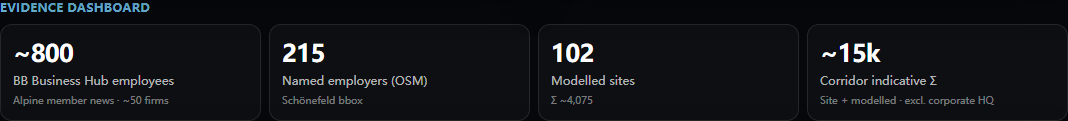
\includegraphics[width=\linewidth,keepaspectratio]{fig-app-dashboard.png}
    \caption*{Evidence dashboard}
  \end{subfigure}
\end{figure}

\begin{figure}[htbp]
  \centering
  
\includegraphics[width=\linewidth,height=0.32\textheight,keepaspectratio]{fig-app-map.png}
  \caption{Live OSM gewerbe layer --- 643 features; named employers highlighted; BB Business Hub anchor.}
\end{figure}

\textbf{Data layers.}

{\small
\begin{tabularx}{\linewidth}{@{}p{2.8cm}Xp{1.4cm}@{}}
\toprule
\textbf{Layer} & \textbf{Business meaning} & \textbf{Cnt} \\
\midrule
OSM gewerbe features & Where economic activity is physically present & 643 \\
Named employers & Firms / outlets we can discuss with Mitglieder & 215 \\
Verified site / registry & Figures we can cite in a board deck & 9 \\
Corporate group match & Brand is present; HQ number is \textit{not} local headcount & 53 \\
Modelled sites & Transparent estimate when no public filing exists & 102 \\
Micro-establishments & Professional services / small retail (range only) & 51 \\
\bottomrule
\end{tabularx}
}

\section*{3.\ Corridor employment model (business view)}
\textit{Purpose:} Give Graf a defensible \textbf{first answer} where public data stops --- without pretending we have confidential HR files.

\textbf{Three-step logic (not a black box).}
\begin{enumerate}
  \setlength{\itemsep}{0.15em}
  \item \textbf{Start with what is published.} Annual reports, member news (BB Hub), and registry excerpts (FBB) anchor the narrative.
  \item \textbf{Classify each named site by business type.} Logistics depots, Werkstätten, Gewerbeparks, airport buildings, and retail units face different typical staffing --- informed by German Mittelstand structure (many small firms, few large plants).
  \item \textbf{Apply a corridor context adjustment.} Locations closer to BER inherit slightly higher job density assumptions --- reflecting the Flughafenregion labour market described in the 2025 FBB/WFBB/IHK study (\textbf{Fachkräftegewinnung} as top challenge, not absent workers).
\end{enumerate}

\textbf{Output format.} For each of the 102 unreported sites we publish a \textbf{range} (conservative to optimistic) and a single \textbf{planning number} inside that range. Example anchors:

\begin{tabularx}{\linewidth}{@{}lrr@{}}
\toprule
\textbf{Location (OSM name)} & \textbf{Planning no.} & \textbf{Range} \\
\midrule
Gewerbepark Schönefeld & 357 & 92--402 \\
Logistikzentrum Airport Park Berlin & 192 & 69--253 \\
Briefzentrum 12 / Logistikzentrum Berlin Südost & 171 & 69--253 \\
Berlin ExpoCenter Airport & 123 & 29--161 \\
\bottomrule
\end{tabularx}

{\small Full 102-row table in \texttt{public/data/graf/employee-predictions.json} and interactive briefing UI.}

\begin{figure}[htbp]
  \centering
  \begin{subfigure}[t]{0.48\textwidth}
    \centering
    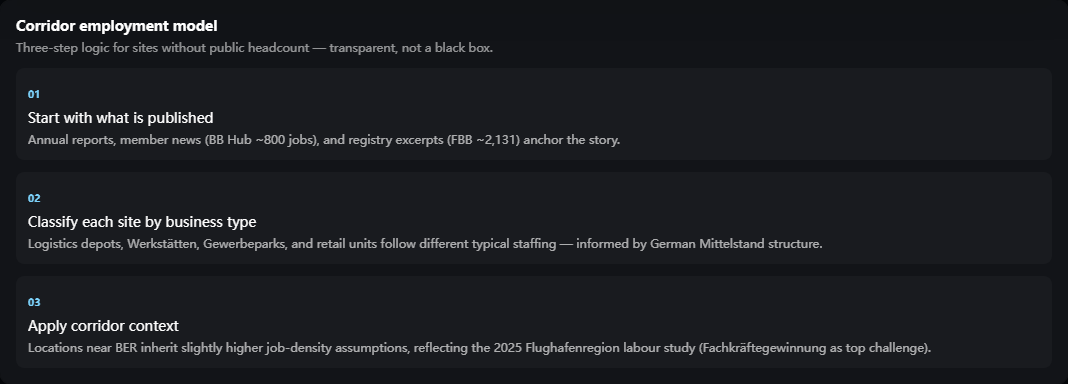
\includegraphics[width=\linewidth,keepaspectratio]{fig-app-model.png}
    \caption*{Corridor model (three steps)}
  \end{subfigure}\hfill
  \begin{subfigure}[t]{0.48\textwidth}
    \centering
    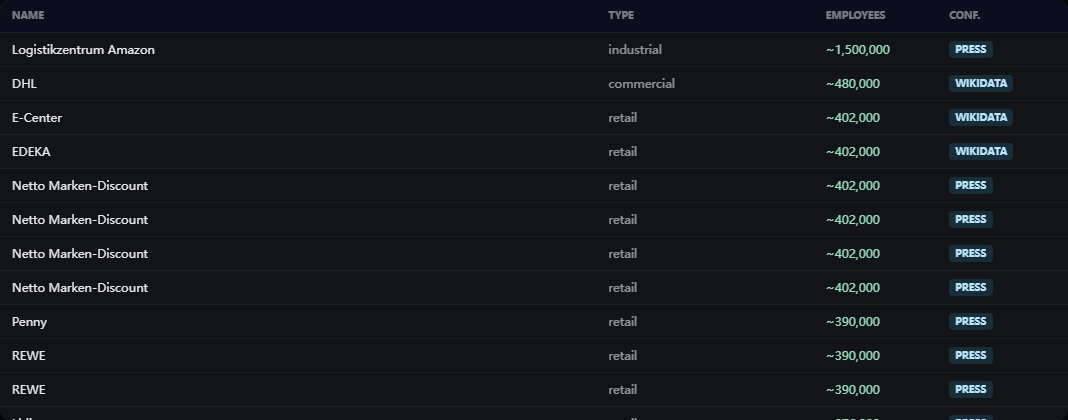
\includegraphics[width=\linewidth,keepaspectratio]{fig-app-table.png}
    \caption*{Employer cross-reference table}
  \end{subfigure}
  \caption{Model explanation and searchable employer table with confidence badges.}
\end{figure}

\textbf{What we deliberately do \textit{not} do.}
\begin{itemize}
  \setlength{\itemsep}{0.1em}
  \item Sum DHL / REWE / Amazon \textbf{global} headcount as if they were Schönefeld site staff.
  \item Present modelled numbers as audited Beschäftigtenzahlen.
  \item Replace a BER+ member validation workshop.
\end{itemize}

\section*{4.\ Answer for Alpine / BER+ board}
\textbf{Is there ``enough manpower''?}
\begin{itemize}
  \setlength{\itemsep}{0.12em}
  \item \textbf{Yes for narrative credibility:} the corridor already hosts hundreds of named gewerbe sites, a validated airport employer ($\sim$2k FBB), and Alpine's own BB Hub proof point ($\sim$800).
  \item \textbf{With caveats for leasing:} tenant recruitment depends on \textbf{Fachkräfte} mobility across $\sim$6M Berlin--Brandenburg --- not only on-site headcount.
  \item \textbf{Next credibility step:} member-validated firm-level numbers for Pilot-1 and 3--5 anchor Mitglieder (Alpine, SEGRO, BUWOG, WFG, Sector Seven).
\end{itemize}

\begin{figure}[htbp]
  \centering
  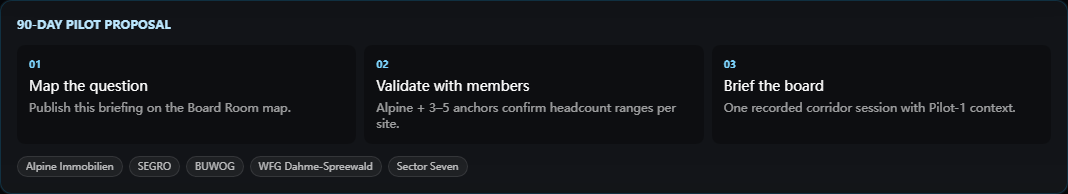
\includegraphics[width=0.92\linewidth,keepaspectratio]{fig-app-pilot.png}
  \caption{Proposed 90-day pilot --- map, validate, brief the board.}
\end{figure}

\section*{5.\ Sources \& limitations}
\textbf{Sources:} OpenStreetMap / Overpass (Schönefeld bbox, June 2026); Alpine / BER+ member news (BB Business Hub, Feb 2025); FBB Geschäftsbericht 2023; FBB/WFBB/IHK Flughafenregion labour study 2025; corporate annual reports / Wikidata for brand-level references only.

\textbf{Limitations:} OSM tags $\neq$ employee counts; model outputs are planning estimates; duplicate OSM nodes for the same facility are split; English briefing with German labour-market terms.

\sectionrule
{\small
\textbf{App route:} \texttt{/beschaeftigung} · \texttt{src/components/GrafBriefingContent.tsx}\\
\textbf{Data pipeline:} \texttt{demos/graf-beschaeftigung-briefing/} → \texttt{scripts/sync-graf-briefing-data.mjs} → \texttt{public/data/graf/}\\
\textbf{Figures:} Playwright captures of the integrated Board Room page (\texttt{capture-screenshots.mjs}).\\
\textbf{Deploy:} \url{https://ber-board-room.vercel.app/beschaeftigung}
}

\end{document}
